\documentclass[12pt]{amsart}

\usepackage{amsmath,amssymb,amscd,amsthm}
\usepackage{hyperref}
\usepackage{enumitem}
\usepackage{graphicx}
\usepackage{tikz-cd}
\usepackage{tikz}
\usetikzlibrary{positioning}
\usetikzlibrary{calc}
\usepackage[a4paper,margin=1in]{geometry}
\usepackage{mathrsfs}
\usepackage{mathtools}

\newcommand{\afunc}[1]{\operatorname{\mathsf{#1}}}

\numberwithin{figure}{section}
\theoremstyle{plain}
\newtheorem{theorem}{Theorem}[section]
\newtheorem{proposition}[theorem]{Proposition}
\newtheorem{lemma}[theorem]{Lemma}
\newtheorem{corollary}[theorem]{Corollary}

\renewcommand{\thesubsection}{\thesection.\Alph{subsection}}

\title[Approaches for Hypercube Power Colourings]{Spectral and Topological Approaches for Hypercube Power Colourings}
\author{Finn Steinke, Rajesh Pereira}
\date{2025/08/08}

\begin{document}

\begin{abstract}
We investigate three prominent graph colouring invariants—the chromatic number $\chi$, achromatic number $\psi$, and $b$-chromatic number $b$ for the $p$th powers of $n$-dimensional hypercube graphs $Q_{n}^{p}$. While the chromatic number has been extensively studied, general bounds for these invariants on hypercube powers remain challenging to obtain. We develop novel algebro-combinatorial methods using spectral graph theory and the Bose–Mesner algebra of the Hamming association scheme to derive lower bounds for $\chi(Q_{n}^{p})$, which extend naturally to $\psi(Q_{n}^{p})$ and $b(Q_{n}^{p})$. In particular, we express eigenvalues in terms of Kravchuk polynomials and present a Hoffman-type bound adapted to this setting. Complementing these spectral results, we introduce an algebro-topological framework based on simplicial complexes associated to hypercube powers, providing connectivity-based bounds based on Lovasz's original findings and exploring equivariant obstructions to colourings of $Q_{n}^{p}$.
\end{abstract}

\maketitle

\tableofcontents

\section{Introduction}
\indent Throughout, all graphs are simple, undirected, and finite. The problem of vertex colouring has remained combinatorially rich for a long period of time. In fact, many notions of graph colouring exist and we will discuss three of the most prominent graph colourings, each with an associated invariant.

\subsection{Proper and optimal colourings} Let $\sqcup$ denote a disjoint union. Let us fix some $k\in\mathbb{N}$. A $k$-colouring of the graph $G$ is a map
\[\mathcal{P}:V(G) \to [k],\]
where $[k] = \{1,2,\dots,k\}$. Then, a colouring is called proper if for all $\{u,v\}\in E(G)$, $\mathcal{P}(u) \neq \mathcal{P}(v)$, where $u,v\in V(G)$. Intuitively, this means that no adjacent vertices can receive the same colour. We will let the set of all proper colourings of $G$ be denoted by $\mathscr{C}(G)$. We can immediately observe the following result for proper colourings.
\begin{proposition}
    Let $G = (V(G), E(G))$ be a graph. A proper $k$-colouring $\mathcal{P}$ induces a partition of $V(G)$ into $k$ subsets of the form
    \[V(G) = \bigsqcup_{i\in[k]}A_{i},\]
    where $A_{i} = \mathcal{P}^{-1}(i)$. Each subset $A_{i}$ is an independent set in $G$.
\end{proposition}
\begin{proof}
    Let $\mathcal{P}: V(G) \to [k]$ be a proper colouring of $G$. For each $i \in [k]$, define
    \[A_{i} = \mathcal{P}^{-1}(i) \coloneq \{ v \in V(G) \mid \mathcal{P}(v) = i \}.\]
    Since $\mathcal{P}$ is a colouring, every vertex $v \in V(G)$ is assigned exactly one colour in $[k]$. Therefore,
    \[V(G) = \bigcup_{i \in [k]} A_i.\]
    Moreover, if $i \neq j$, then $A_i \cap A_j = \emptyset$ because a vertex cannot receive two distinct colours. Hence, $\{A_i\}_{i \in [k]}$ is a partition of $V(G)$.\\
    \indent Next, we show that each $A_{i}$ is an independent set. Suppose, for contradiction, that there exist $u,v \in A_{i}$ such that $\{u,v\} \in E(G)$. Then, by definition of $A_{i}$, $\mathcal{P}(u) = \mathcal{P}(v) = i$. But since $\{u,v\} \in E(G)$ and $\mathcal{P}$ is proper, we must have $\mathcal{P}(u) \neq \mathcal{P}(v)$, a contradiction. Therefore, no such edge exists, and each $A_{i}$ is an independent set.
\end{proof}
\indent We define the chromatic number of $G$ as
\[\chi(G) = \min\{k\:|\:\mathscr{C}(G)\neq\emptyset\},\]
where each colouring in $\mathscr{C}(G)$ is of the form $\mathcal{P}:V(G) \to [k]$ by definition. Any proper colouring $\mathcal{P}\in\mathscr{C}(G)$ with $\chi(G)$ colours is known as an optimal colouring of $G$. For a more traditional definition of optimal colouring, see \cite{West01}. The chromatic number is the most well-studied graph colouring invariant, with wide-reaching applications in many areas of pure mathematics. Since $\chi$ is generally $\afunc{NP}$-hard to compute, this motivates our primary focus of the paper, namely the bounding of $\chi$ for a specific graph family we will introduce in section $1$.D.\\
\indent To make precise the definition of a proper $k$-colouring of $G$, we often describe it as a graph homomorphism from $G$ to the complete graph on $k$ vertices $K_{k}$. We recall that a graph homomorphism is a map $\phi:G\to H$ such that for all $\{u,v\}\in E(G)$, there exists $\{\phi(u), \phi(v)\}\in E(H)$. Then, a colouring $\mathcal{P}$ is precisely a graph homomorphism such that $\mathcal{P}:G\to K_{k}$. We summarize the relationship with the following diagram
\[\begin{tikzcd}
G \arrow[r,"\phi"] \arrow[dr, "\mathcal{P}"'] & H \arrow[d, "\mathcal{Q}"] \\ & K_k \end{tikzcd}\]
which commutes if and only if $\mathcal{P} = \mathcal{Q}\circ\phi$.\\
\indent A rather important result with regard to the chromatic number is given in \cite{Brooks41} and is commonly known as Brooks' theorem, which we will restate as a lemma.
\begin{lemma}
    Let $G$ be a connected graph with maximum degree $\Delta(G)$. If $G$ is neither a complete graph nor an odd cycle, then
    \[\chi(G) \leq \Delta(G).\]
    In all cases, we have the trivial bound $\chi(G) \leq \Delta(G) + 1$.
\end{lemma}
\begin{proof}
    Given in \cite{Brooks41}.
\end{proof}
\indent For any graph $G$, let us consider a subset $C\subseteq V(G)$. If for all distinct pairs $u, v \in C$ there exists $\{u,v\}\in E(G)$, then $C$ is known as a clique of $G$. Equivalently, the subgraph of $G$ induced by $C$ is a complete graph. This leads us to another key insight for bounding $\chi$ for general graphs.
\begin{proposition}
    For any graph $G$, the chromatic number satisfies
    \[\chi(G) \geq \omega(G),\]
    where $\omega(G)$ is the size of the largest clique in $G$.
\end{proposition}
\begin{proof}
    Let $G$ be a graph and let $\omega(G)$ denote the size of the largest clique in $G$. By definition, a clique of size $\omega(G)$ consists of $\omega(G)$ vertices such that every pair of distinct vertices is adjacent. In any proper coloring of $G$, adjacent vertices must receive different colors. Therefore, all vertices of this clique must be assigned distinct colors. Consequently, any proper coloring of $G$ requires at least $\omega(G)$ colors, and hence
    \[\chi(G) \geq \omega(G).\]
\end{proof}
\begin{proposition}
    For any graph $G$, the chromatic number satisfies
    \[\omega(G)\leq\chi(G)\leq\Delta(G)+1.\]
\end{proposition}
\begin{proof}
    Follows directly from lemma 1.2. and proposition 1.3.
\end{proof}
\indent Finally, $\chi$ was found to have a spectral lower bound, as given by Hoffman's theorem in \cite{Hof03}, another theorem we will rewrite as a lemma.
\begin{lemma}
    For any graph $G$, the chromatic number satisfies
    \[\chi(G) \geq 1 + \frac{\operatorname{\max}\limits_{1\leq i \leq |V(G)|}\{\lambda_{i}\in\operatorname{Spec(A(G))}\}}{|\operatorname{\min}\limits_{1\leq i \leq |V(G)|}\{\lambda_{i}\in\operatorname{Spec(A(G))}\}|},\]
    where $A(G)$ is the adjacency matrix of $G$ and where $\lambda_{i}$ are the corresponding eigenvalues of $A(G)$.
\end{lemma}
\begin{proof}
    Given in \cite{Hof03}.
\end{proof}
\subsection{Complete colourings} A complete $k$-colouring of $G$ is a proper colouring $\mathcal{P}$ such that for every pair of distinct colours $i, j\in[k]$ with $i\neq j$, there exists $\{u,v\}\in E(G)$ where $\mathcal{P}(u) = i$ and $\mathcal{P}(v) = j$. Intuitively, this means that every pair of colours appears on adjacent vertices somewhere in the graph, and no colour is “isolated” from the others.\\
\indent We can introduce the idea of complete $k$-colouring with more precision using an equivalence relation. Given a proper $k$-colouring $\mathcal{P}\in\mathscr{C}(G)$, we define the equivalence relation $\sim_{\mathcal{P}}$ on $V(G)$ such that
\[\sim_{\mathcal{P}}\:\coloneq\left\{(u,v)\in V(G)\times V(G)\:\middle|\:\mathcal{P}(u) = \mathcal{P}(v)\right\},\]
where the equivalence classes of the equivalence relation are the colour classes of $\mathcal{P}$, given by $A_{i} = \mathcal{P}^{-1}(i)$, where $i\in[k]$. Now, we define the quotient graph $G/\!\sim_{\mathcal{P}}$, where
\[V(G/\!\sim_{\mathcal{P}}) = \{A_{1},A_{2},\dots,A_{k}\},\]
and where $\{A_{i},A_{j}\}\in E(G/\!\sim_{\mathcal{P}})$ if and only if there exist $u \in A_{i}$ and $v\in A_{j}$ such that $\{u,v\}\in E(G)$. It follows that if $\mathcal{P}$ is a complete $k$-colouring, then
\[G/\!\sim_{\mathcal{P}}\:\cong K_{k}.\]
\indent We can relate complete $k$-colouring to graph homomorphisms as before.
\begin{proposition}
    Let $G = (V(G), E(G))$ be any graph and let $\mathcal{P}\in\mathscr{C}(G)$ be a proper $k$-colouring of $G$. Then, $\mathcal{P}$ is a surjective graph homomorphism such that $\mathcal{P}: G\to K_{k}$.
\end{proposition}
\begin{proof} 
    Let $\mathcal{P} : V(G) \to [k]$, where the vertices of $K_{k}$ are identified with the set $[k]$. For each $i \in [k]$, we define the colour class
    \[A_{i} = \mathcal{P}^{-1}(i) \coloneq \{ v \in V(G) \mid \mathcal{P}(v) = i \}.\]
    Since $\mathcal{P}$ is a proper colouring, by definition for all $\{u,v\} \in E(G)$ we have $\mathcal{P}(u) \neq \mathcal{P}(v)$. Hence, $\{\mathcal{P}(u), \mathcal{P}(v)\}$ is an edge in $K_{k}$, because $K_{k}$ is complete and contains all edges between distinct vertices. Thus, $\mathcal{P}$ preserves adjacency, and therefore it is a graph homomorphism.\\
    \indent Furthermore, $\mathcal{P}$ uses exactly $k$ colours, so every $i \in [k]$ has a non-empty preimage $A_{i}\neq\emptyset$. This implies $\mathcal{P}$ is surjective on vertices, and is thus a surjective graph homomorphism.
\end{proof}
\indent We define the achromatic number of $G$ as
\[\psi(G) = \max\{k\:|\:\mathscr{C}(G)\neq\emptyset, G/\!\sim_{\mathcal{P}}\:\cong K_{k}\},\]
where any colouring $\mathcal{P}\in\mathscr{C}(G)$ and $\mathcal{P}$ defines $\sim_{\mathcal{P}}$. It is the case that finding $\psi$ generally is $\afunc{NP}$-hard, as was the case with $\chi$. A trivial, yet important result for the achromatic number is immediately observable.
\begin{proposition}
    For any graph $G$, the achromatic number satisfies
    \[\psi(G) \geq \chi(G).\]
\end{proposition}
\begin{proof}
    Let $G$ be a graph. By definition, any complete colouring $\mathcal{P}$ of $G$ must be proper. Since $\chi(G)$ is the minimum number of colours required for a proper colouring, the result follows.
\end{proof}
\indent We find a rather interesting result for the upper bound on $\psi$ in general.
\begin{theorem}
For any graph $G$, there is no upper bound on $\psi(G)$ that depends on both the spectrum of $A(G)$ and $\Delta(G)$.
\end{theorem}
\begin{proof}
    For each $k \in \mathbb{N}$, define $G_{k}$ as follows: start with a star $K_{1,k}$, and replace each leaf by a path of length 2. Then $G_{k}$ is a tree on $2k + 1$ vertices. We have:
    \[\Delta(G_k) = 2, \quad \operatorname{Spec}(A(G_{k})) \subseteq [-2,2].\]
    Let $v_{1}, \dots, v_{k}$ be the $k$ leaves (endpoints of the paths). Assign each $v_{i}$ a distinct colour, and extend this to a proper colouring in which every pair of colours appears on an edge. Then $\psi(G_{k}) \geq k$. Hence, $\psi(G_{k}) \to \infty$ while $\Delta(G_{k})$ and the spectrum of $A(G_{k})$ remain bounded. No function of these can bound $\psi(G)$.
\end{proof}
\subsection{$b$-colourings} A $b$-colouring of $G$ with $k$ colours is a proper colouring $\mathcal{P}$ such that for any colour class $A_{i}$ there exists at least one $b$-vertex $v_{i}\in A_{i}$ satisfying
\[N(v_{i})\cap A_{j} \neq \emptyset\]
for all $j \neq i$, where $i,j\in[k]$ and $N(v_{i}) = \left\{u\in V(G)\:\middle|\:\{v_{i}, u\}\in E(G)\right\}$. Intuitively, this means every colour class $A_{i}$ contains a vertex adjacent to at least one vertex of every other colour class. We can immediately find a result through the perspective of graph homomorphisms as with proper and complete colourings.
\begin{proposition}
    A $b$-colouring of $G$ with $k$ colours exists if and only if there is a graph homomorphism $\mathcal{P}: G \to K_{k}$ such that for every $i \in [k]$, there exists a vertex $v \in \mathcal{P}^{-1}(i)$ satisfying
    \[\mathcal{P}(N(v))=[k]\setminus\{i\}.\]
\end{proposition}
\begin{proof}
    Let $G$ be a graph. $(\Rightarrow)$ Suppose $G$ admits a $b$-colouring with $k$ colours. We define $\mathcal{P}: G \to K_{k}$ by $\mathcal{P}(u) = i$ if $u \in A_{i}$. Properness of the colouring implies $\mathcal{P}$ is a graph homomorphism. For each $i$, the $b$-colouring condition guarantees a vertex $v_{i} \in A_{i}$ whose neighbourhood intersects every other colour class, hence $\mathcal{P}(N(v_{i})) = [k]\setminus{i}$.\\
    \indent $(\Leftarrow)$ Conversely, if such a homomorphism exists, define the colour classes as $A_{i} = \mathcal{P}^{-1}(i)$. Properness follows from $\mathcal{P}$ being a homomorphism. The local surjectivity property guarantees each class contains a $b$-vertex. Thus, the colouring is a $b$-colouring.
\end{proof}
\indent We also notice another result, this one about the maximum degree of any $b$-coloured graph.
\begin{proposition}
    Let $G=(V(G), E(G))$ be a graph. If $G$ admits a $b$-colouring with $k$ colours, then
    \[\Delta(G) \geq k-1.\]
\end{proposition}
\begin{proof}
    Let $G$ be a graph where $v\in V(G)$ is a $b$-vertex in some colour class. By definition, $v$ must have a neighbour in every other colour class, where there are $k-1$ colour classes remaining. Therefore, $\mathrm{deg}(v) \geq k-1$, and since $\mathrm{deg}(v)\leq\Delta(G)$, the conclusion follows directly.
\end{proof}
\indent We define the $b$-chromatic number of $G$ as
\[b(G) = \max\left\{k\:\middle|\:\mathcal{P}\in\mathscr{C}(G), \forall i\in[k], \exists v\in\mathcal{P}^{-1}(i) \text{ such that } \mathcal{P}(N(v)) = [k]\setminus\{i\}\right\},\]
where $N(v)$ is the open neighbourhood of a vertex, as defined previously. As with $\chi$ and $\psi$, it was shown in \cite{IrvMan99} that finding $b$ for general $G$ is $\afunc{NP}$-hard. It was also shown in the same text that there is only a superficial similarity between $b(G)$ and $\Gamma(G)$, the Grundy number, and that neither bounds or impacts the other in any meaningful way. Indeed, we can apply the same trivial result found for $\psi$ to $b$.
\begin{proposition}
    For any graph $G$, the $b$-chromatic number satisfies
    \[b(G) \geq \chi(G)\]
\end{proposition}
\begin{proof}
    Nearly identical to the proof of proposition 1.7.
\end{proof}
\indent Moreover, similarly to $\chi$, an upper bound in terms of $\Delta(G)$ can be generally constructed using proposition 1.10.
\begin{corollary}
    For any graph $G$, the $b$-chromatic number satisfies
    \[b(G) \leq \Delta(G) + 1.\]
\end{corollary}
\begin{proof}
    Let $G$ be a graph. Then, by definition of $b$, we know that $b(G) = k$ for the maximal $b$-colouring, and hence
    \[\Delta(G) \geq b(G) - 1 \implies b(G)\geq\Delta(G) + 1.\]
\end{proof}
\begin{proposition}
    For any graph $G$, the $b$-chromatic number satisfies
    \[\chi(G) \leq b(G) \leq \Delta(G) + 1.\]
\end{proposition}
\begin{proof}
    Follows directly from proposition 1.11. and corollary 1.12.
\end{proof}
\indent Let $\mathscr{A}(G)$ be the set of all colourings of $G$, proper and improper. It should be noted that the formal definition of $b$-colouring, as in \cite{IrvMan99}, requires the definition of a relation $R_{G}$ such that
\[R_{G} \coloneq \left\{(\mathcal{P},\mathcal{Q}) \in \mathscr{A}(G)\times\mathscr{A}(G)\:\middle|\:\mathcal{P}^{-1}(i) = \textstyle\bigsqcup_{j\in S_{i}}\mathcal{Q}^{-1}(j), \forall i\in [k]\right\}\]
where $\mathcal{P}:V(G) \to [k]$, $\mathcal{Q}:V(G)\to[k+1]$, and where $\{S_{i}\}_{i=1}^{k}$ is a partition of $[k+1]$. The transitive closure of $R_{G}$, given by $R_{G}^{*}$, induces a strict ordering, where we let
\[b(G) \coloneq \max \left\{ k \in\mathbb{N} \:\middle|\:\mathcal{P} \in \mathscr{C}(G),\: \mathcal{P} \text{ is } R_G^*\text{-minimal} \right\}.\]
Any proper colouring $\mathcal{P}$ on $G$ which is $R_{G}^{*}$-minimal is said to be a $b$-colouring of $G$. This was introduced as a refinement to the complete colouring, which was given a similar relational definition. We present this definition for clarity for the origin of $b$-colouring, but the earlier definition is far more concise.\\
\indent The next section will focus on the family of graphs we will be finding $\chi, \psi, b$ bounds for.
\subsection{Hypercube graphs and $p$th powers}
\indent We define the hypercube graph $Q_{n}$ using a vector space, where 
\[V(Q_{n}) \coloneqq\mathbb{F}_{2}^{n},\quad E(Q_{n}) \coloneqq\left\{\{\mathbf{x},\mathbf{y}\}\subseteq\mathbb{F}_{2}^{n}\:\middle|\:d_{H}(\mathbf{x},\mathbf{y}) = 1,\right\}\]
such that the Hamming metric $d_{H}$ is equipped with a vector-based definition, analogous to the $\ell^{1}$ norm, 
\[d_{H}(\mathbf{x},\mathbf{y})\coloneq\sum_{i=1}^{n}|x_{i} - y_{i}|.\]
\indent We observe some important result for hypercube graphs and their colourings.
\begin{proposition}
    Every hypercube graph $Q_{n}$ is bipartite.
\end{proposition}
\begin{proof}
    Let $Q_{n}$ be the hypercube graph of vector length $n\geq 2$. We define the sets 
    \[U \coloneq \left\{\mathbf{x}\in\mathbb{F}_{2}^{n}\:\middle|\:\textstyle\sum_{i=1}^{2}x_{i} \equiv 0 \:(\!\!\!\!\!\!\mod 2)\right\},\]
    and
    \[W\coloneq\left\{\mathbf{y}\in\mathbb{F}_{2}^{n}\:\middle|\:\textstyle\sum_{i=1}^{2}y_{i} \equiv 1 \:(\!\!\!\!\!\!\mod 2)\right\}.\]
    If $\mathbf{x}$ and $\mathbf{y}$ are adjacent, only one coordinate will differ between them, so their coordinate sums will differ in parity. Since $U\cup W = \mathbb{F}_{2}^{n}$, $U\cap W = \emptyset$, and $\emptyset \notin \{U, W\}$, we have shown that $\{U, W\}$ forms a valid partition of $\mathbb{F}_{2}^{n}$, and hence the conclusion follows.
\end{proof}
\indent This leads us directly to a corollary.
\begin{corollary}
    For all $n\geq 2$, the hypercube graph $Q_{n}$ satisfies
    \[\chi(Q_{n}) = 2.\]
\end{corollary}
\begin{proof}
    Follows directly from  proposition 1.14.
\end{proof}
\indent We then define the $p$th power of the hypercube graph $Q_{n}^{p}$ such that
\[V(Q_{n}^{p}) \coloneq V(Q_{n}) = \mathbb{F}_{2}^{n},\quad E(Q_{n}^{p}) \coloneq\left\{\{\mathbf{x}, \mathbf{y}\}\subseteq\mathbb{F}_{2}^{n}\:\middle|\:1\leq d_{H}(\mathbf{x}, \mathbf{y}) \leq p\right\},\]
where $1\leq p\leq n$. It is trivial that $Q_{n}^{1} \cong Q_{n}$, and equally trivial that $Q_{n}^{n} \cong K_{2^{n}}$, making cases where $p=1$ and $p=n$ generally uninteresting to study for powers. For this reason, the first nontrivial case is $Q_{3}^{2}$, a typical construction of which is given in \ref{fig:q32}.
\begin{figure}[h]
  \centering
    \vspace{-1.5cm}
    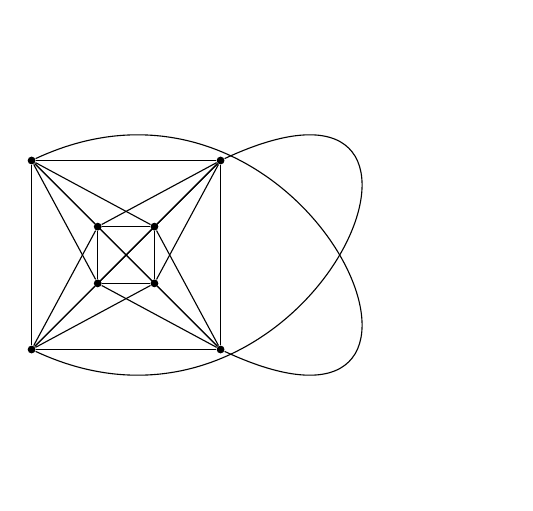
\begin{tikzpicture}[scale=2.4, every node/.style={circle, fill=black, inner sep=1pt}, font=\small]
    \node (000) at (0,1) {}; 
    \node (001) at (0,0) {}; 
    \node (100) at (1,1) {}; 
    \node (101) at (1,0) {};   
    \node (010) at (0.35,0.65) {};
    \node (011) at (0.35,0.35) {};
    \node (110) at (0.65,0.65) {};
    \node (111) at (0.65,0.35) {};
    \foreach \i/\j in {
      000/001, 000/010, 000/100, 000/011, 000/101, 000/110,
      001/010, 001/011, 001/100, 001/101, 001/111,
      010/011, 010/100, 010/110, 010/111,
      011/100, 011/101, 011/110, 011/111,
      100/101, 100/110, 100/111,
      101/110, 101/111,
      110/111}
      \draw (\i) -- (\j);
    \draw (000) .. controls +(1.5,0.7) and +(1.5,-0.7) .. (101);
    \draw (001) .. controls +(1.5,-0.7) and +(1.5,0.7) .. (100);
    \end{tikzpicture}
    \vspace{-1.5cm}
  \caption{Typical construction of $Q_{3}^{2}$}
  \label{fig:q32}
\end{figure}

\indent We give a trivial result for $\chi(Q_{n}^{p})$ that follows a general result for graphs.
\begin{proposition}
    Let $G$ be a graph and $H\subseteq G$ a subgraph. Then, the chromatic numbers of both $G$ and $H$ satisfy
    \[\chi(H) \leq \chi(G).\]
\end{proposition}
\begin{proof}
    Let $G$ be a graph with subgraph $H$. Suppose there exists a proper $k$-colouring of $G$, denoted $\mathcal{P}$. We then define the restriction map
    \[\mathrm{res}_{H}:\mathscr{C}(G) \to\mathscr{C}(H),\]
    where for any colouring $\mathcal{P}$ of $G$, we set
    \[\mathrm{res}_{H}(\mathcal{P}) = \mathcal{P}|_{V(H)}.\]
    Then, since $E(H) \subseteq E(G)$, if $\mathcal{P}$ is proper on $G$, then $\mathcal{P}|_{V(H)}$ must be proper on $H$. Since $\mathcal{P}$ uses $k$ colours, then $\mathcal{P}|_{V(H)}$ will use at most $k$ colours, meaning
    \[\chi(H) \leq k = \chi(G).\]
\end{proof}
\indent Extending to graph powering, we find a similar result.
\begin{corollary}
    Let $G$ be a graph and $G^{p}$ its $p$th power, based on the standard graph metric $d_{G}$. Then, the chromatic numbers of both $G$ and $G^{p}$ satisfy
    \[\chi(G) \leq \chi(G^{p}).\]
\end{corollary}
\begin{proof} Let $G = (V,E)$ be a graph. It is enough to show that $G\subseteq G^{p}$, where $G$ is a subgraph. Recall that $G^{p}$ is defined on the same vertex set $V(G)$, where two vertices $u,v$ are adjacent in $G^{p}$ if and only if $d_{G}(u,v) \leq p$. In particular, if $u$ and $v$ are adjacent in $G$, then $d_{G}(u,v) = 1 \leq p$, so every edge of $G$ is also an edge of $G^{p}$. Therefore, 
\[E(G) \subseteq E(G^{p}),\] 
meaning $G$ is a subgraph of $G^{p}$.
\end{proof}
\begin{proposition}
    For all $n\geq 2$, $1\leq p\leq n$, the $p$th power hypercube graph $Q_{n}^{p}$ satisfies
    \[\chi(Q_{n}^{p}) \geq 2.\]
\end{proposition}
\begin{proof}
    Follows directly from corollary 1.15. and corollary 1.17.
\end{proof}
\indent \cite{Francis17} presented some strong results for certain values of $b(Q_{n}^{p})$, $\chi(Q_{n}^{p})$, and $\omega(Q_{n}^{p})$. These results highly useful for most if not all graphs $Q_{n}^{p}$, and were found combinatorially. We list four of the text's results below, as they will be important to compare with our results later.
\begin{theorem}
    For all $n\geq 2$,
    \[b(Q_{n}^{n-1}) = 2^{n-1}.\]
\end{theorem}
\begin{proof}
    Given in \cite{Francis17}.
\end{proof}
\begin{theorem}
    For all $n\geq 2$,
    \[b(Q_{n}^{\left\lfloor\frac{n}{2}\right\rfloor}) = 2^{n-1}.\]
\end{theorem}
\begin{proof}
    Given in \cite{Francis17}.
\end{proof}
\begin{theorem}\normalfont
\begin{enumerate}[label=(\roman*)]
    \item\textit{ For all $n \geq 3$ and $1 \leq p \leq n-1$,
    \[
        \omega(Q_{n}^{p}) =
        \begin{cases}
            \sum_{i=0}^{\frac{p}{2}}\binom{n}{i}, & \text{if } p \text{ is even},\\[6pt]
             2\sum_{i=0}^{\frac{p-1}{2}}\binom{n-1}{i}, & \text{if } p \text{ is odd,}
        \end{cases}
    \]}
    \item\textit{ For all $n \geq 2$ and $\left\lfloor \frac{n}{2}\right\rfloor < p < n-1$,
    \[
        2^{n-1} \leq b(Q_{n}^{p}) \leq 2^{n-1} + \left\lfloor \frac{\omega(Q_{n}^{p})}{2}\right\rfloor.
    \]}
\end{enumerate}
\end{theorem}
\begin{proof}
    Given in \cite{Francis17}.
\end{proof}
\begin{theorem}
    For all $n\geq 2$ and $\left\lceil\frac{2(n-1)}{3}\right\rceil \leq p \leq n-1$,
    \[\chi(Q_{n}^{p}) = 2^{n-1}.\]
\end{theorem}
\begin{proof}
    Given in \cite{Francis17}.
\end{proof}
\indent In fact, we can state a quick result that builds on theorem 1.21.(i).
\begin{corollary}
    For all $n\geq 3$ and $1\leq p \leq n-1$,
    \[\chi(Q_{n}^{p}) \geq 
    \begin{cases}
        \sum_{i=0}^{\frac{p}{2}}\binom{n}{i}, & \text{if } p \text{ is even},\\[6pt]
             2\sum_{i=0}^{\frac{p-1}{2}}\binom{n-1}{i}, & \text{if } p \text{ is odd.}
    \end{cases}\]
\end{corollary}
\begin{proof}
    Follows directly from proposition 1.3. and theorem 1.21.(i).
\end{proof}
\indent The specific interest of this text is finding general bounds for $\chi(Q_{n}^{p})$ using novel methods, expanding to discuss $\psi(Q_{n}^{p})$ and $b(Q_{n}^{p})$ whenever possible. The methods of interest will be presented in the following sections as they are used.
\section{Algebro-combinatorial results}
\indent We introduce the Kravchuk polynomials, first presented in \cite{kravchuk1929} to use in this section's main result. Let $\mathcal{K}_{i}(x;n,q)$ denote the $i$th Kravchuk polynomial of $x$, where we define
\[\mathcal{K}_{i}(x;n, q) = \sum_{j=0}^{i}(-1)^{j}(q-1)^{i-j}\binom{x}{j}\binom{n-x}{i-j},\]
where $n\in\mathbb{N}$, $q$ is a prime power, and $i\in[n]$. In particular, we will make use of the case where $q=2$, where the polynomials reduce to
\[\mathcal{K}_{i}(x;n,2) \eqqcolon \mathcal{K}_{i}(x;n) = \sum_{j=0}^{i}(-1)^{j}\binom{x}{j}\binom{n-x}{i-j}.\]
\indent We define an $n$-class Hamming scheme as the ordered pair $(\mathbb{F}_{2}^{n}, \{R_{j}\}_{j=0}^{n})$, where 
\[R_{j}\coloneq \{(\mathbf{x},\mathbf{y})\in\mathbb{F}_{2}^{n}\times\mathbb{F}_{2}^{n}\:|\:d_{H}(\mathbf{x},\mathbf{y}) = j\}.\]
To do this, we define $(A_{j})_{\mathbf{x},\mathbf{y}}\coloneq
\begin{cases}
        1, & \text{if } (\mathbf{x}, \mathbf{y}) \in R_{j} \\
        0, & \text{otherwise,}
\end{cases}$
such that $\{A_{j}\}_{j=0}^{n}$ generate the Bose-Mesner algebra $\mathcal{A} = \mathrm{span}_{\mathbb{R}}\bigl\{\{A_{j}\}_{j=0}^{n}\bigr\}\subseteq\mathbb{R}^{n\times n}$. There are certain key facts about the Bose-Mesner algebra we discuss, taken from \cite{BI84}.
\begin{proposition}
    Let $(X, \{R_{j}\}_{j=0}^{n})$ be an $n$-class association scheme. Then, the Bose-Mesner algebra $\mathcal{A}$ generated by the associated $\{A_{j}\}_{j=0}^{n}$ satisfies the following:\normalfont
    \begin{enumerate}[label=(\roman*)]
        \item\textit{$\mathcal{A}$ is a commutative, semisimple subalgebra of $\mathbb{R}^{X \times X}$,}
        \item\textit{The matrices $\{A_{j}\}$ are real symmetric and simultaneously diagonalizable,}
        \item\textit{There exists a unique basis $\{J_{0}, \dots, J_{n}\}$ of $\mathcal{A}$ consisting of pairwise orthogonal idempotents (i.e., $J_{i} J_{j} = \delta_{ij} J_{i}$ and $\sum_{i=0}^{n} J_{i} = I$, where $\delta_{ij}$ denotes the Kronecker delta).}
    \end{enumerate}
\end{proposition}
\begin{proof}
    Given in \cite{BI84}.
\end{proof}
\indent We also know a key fact about the eigenvalues of each $A_{j}$.
\begin{lemma}
    Let $(\mathbb{F}_{2}^{n}, \{R_{j}\}_{j=0}^{n})$ be the $n$-class Hamming scheme with corresponding Bose-Mesner algebra $\mathcal{A} =\mathrm{span}_{\mathbb{R}}\bigl\{\{A_{j}\}_{j=0}^{n}\bigr\}$. Then the eigenvalues of $A_{j}$ satisfy
    \[A_{j}\mathbf{v}_{k} = \mathcal{K}_{j}(k; n) \mathbf{v}_{k},\]
    where $\mathbf{v}_{k}\in\mathrm{Im}(J_{k})$ with $0\leq k\leq n$, where $J_{k}$ is a primitive idempotent in $\mathcal{A}$.
\end{lemma}
\begin{proof}
    Given in \cite{BI84}.
\end{proof}
\indent We are now ready for our main result of the section.
\begin{theorem}
For all $n\geq 1$ and $1\leq p \leq n$,
\[\chi(Q_{n}^{p}) \geq 1 + \dfrac{\sum_{i=1}^{p}\binom{n}{i}}{- \min\limits_{0\leq k\leq n}\left\{\sum_{i=1}^{p}\sum_{j=0}^{i}(-1)^{j}\binom{k}{j}\binom{n-k}{i-j}\right\}}.\]
\end{theorem}
\begin{proof}
    \indent Let $(\mathbb{F}_{2}^{n}, \{R_{i}\}_{i=0}^{n})$ be the Hamming scheme. By proposition 2.1.(i,iii), the adjacency matrices $\{A_{i}\}_{i=0}^{n}$ generate a commutative, semisimple subalgebra of $\mathbb{R}^{2^{n} \times 2^{n}}$ with a basis of primitive orthogonal idempotents $\{J_{k}\}_{k=0}^{n}$. Since these matrices are simultaneously diagonalizable by proposition 2.1.(ii), there exists a common orthonormal basis of eigenvectors $\{\mathbf{v}_{k}\}_{k=0}^{n}$ such that each $\mathbf{v}_{k} \in \mathrm{Im}(J_{k})$. We also know that 
    \[A(Q_{n}^{p}) = \sum_{i=1}^{p}A_{i}.\]
    By lemma 2.2., we find
    \[A(Q_{n}^{p})\mathbf{v}_{k} = \left(\sum_{i=1}^{p}\mathcal{K}_{i}(k; n)\right)\mathbf{v}_{k},\]
    where $\lambda_{k} = \sum_{i=1}^{p}\mathcal{K}_{i}(k; n)$ for $0\leq k\leq n$. The largest eigenvalue is given by
    \[\lambda_{0} = \sum_{i=1}^{p}\binom{n}{i},\]
    and the smallest by
    \[\min\limits_{0\leq k\leq n}\lambda_{k}.\]
    Since $A_{i}$ are real symmetric matrices, 
    \[\mathrm{tr}\bigl(A(Q_{n}^{p})\bigr) = \sum_{i=1}^{p}\mathrm{tr}(A_{i}) = 0.\]
    However, we know that
    \[\sum_{k=0}^{n}\dim\bigl(\mathrm{Im}(J_{k})\bigr)\lambda_{k} = 0,\]
    where $\lambda_{0} >0$, then $\min\limits_{0\leq k\leq n}\lambda_{k} < 0$ to satisfy the trace requirement. Finally, applying lemma 1.5. and writing out the Kravchuk polynomials explicitly, the conclusion follows.
\end{proof}
\indent It can be noted that the above result can be proved without the use of the Kravchuk polynomials, instead relying on the machinery of Hadamard matrices and counting principles. We give this proof below, after a lemma.
\begin{lemma}
    Let $H_{2} = \begin{bmatrix}
    1 & 1 \\
    1 & -1
    \end{bmatrix}$ be the $2\times 2$ Hadamard matrix. Then, for all $n\geq 1$, a $2^{n}\times 2^{n}$ Hadamard matrix satisfies
    \[H_{2^{n}} = H_{2}^{\otimes n},\]
    where $\otimes$ denotes the Kronecker product.
\end{lemma}
\begin{proof}
    We prove the lemma using weak induction. The base case, $n=1$, trivially gives us $H_{2^{1}} = H_{2}^{\otimes 1} = \begin{bmatrix}
    1 & 1 \\
    1 & -1
    \end{bmatrix}$. We assume that the conclusion holds for some $k \in \mathbb{N}$, where $k\leq n$. Thus, we take the inductive step, where $n= k+1$. Here, by results concerning construction of Hadamard matrices in \cite{Sylvester1867}, we find that $H_{2^{k+1}} = \begin{bmatrix}
    H_{2^{k}} & H_{2^{k}} \\
    H_{2^{k}} & -H_{2^{k}}
    \end{bmatrix}$, and by definition of the Kronecker product
    \[\begin{bmatrix}
    H_{2^{k}} & H_{2^{k}} \\
    H_{2^{k}} & -H_{2^{k}}
    \end{bmatrix} = \begin{bmatrix}
    1\cdot H_{2^{k}} & 1\cdot H_{2^{k}} \\
    1\cdot H_{2^{k}} & (-1)\cdot H_{2^{k}}
    \end{bmatrix} = H_{2}\otimes H_{2}^{\otimes k} = H_{2}^{\otimes(k+1)},\]
    and therefore the conclusion follows.
\end{proof}
This directly leads us to the following alternative proof of theorem 2.3.
\begin{proof}
    \textit{of \textbf{Theorem 2.3.}} Let $(\mathbb{F}_{2}^{n}, \{R_{i}\}_{i=0}^{n})$ be the Hamming scheme. We observe that
    \[A_{i} = \sum_{S \subseteq [n],|S|=i} \bigotimes_{j=1}^n M_j^{S},  \text{ where } M_j^{S} = 
    \begin{cases}
        J_{1} = \begin{bmatrix}0 & 1 \\ 1 & 0 \end{bmatrix}, & \text{if } j \in S, \\
        I_{2} = \begin{bmatrix}1 & 0 \\ 0 & 1 \end{bmatrix}, & \text{if } j \notin S.
        \end{cases}\]
    The $2\times 2$ Hadamard matrix $H_{2}$ diagonalizes both $I_{2}$ and $J_{1}$ simultaneously with eigenvalues:
    \[\mathrm{Spec}(I_2) = \{1,1\}, \quad \mathrm{Spec}(J_1) = \{1,-1\}.\]
    Therefore by constructing $H_{2^{n}}$ using lemma 2.4., the $2^{n} \times 2^{n}$ Hadamard matrix diagonalizes all $A_{i}$ simultaneously. An eigenvector of $H_{2^{n}}$ corresponds to a vector $\mathbf{k} \in \mathbb{F}_{2}^{n}$ with Hamming weight $k = |\mathbf{k}|$, where on coordinate $j$ the eigenvalue is
    \[\lambda_j = 
    \begin{cases}
        1, & \text{if }k_{j} = 0, \\
        -1, & \text{if }k_{j} = 1.
    \end{cases}\]
    For a fixed $\mathbf{k}$, the eigenvalue $\lambda_i(k)$ of $A_{i}$ is then
    \[\lambda_i(k) = \sum_{S \subseteq [n], |S|=i} \prod_{j \in S} (-1)^{k_{j}} = \sum_{S \subseteq [n], |S|=i} (-1)^{|S \:\cap\: \mathrm{supp}(\mathbf{k})|},\]
    where $\mathrm{supp}(\mathbf{k}) \coloneq \{ j\:|\: k_{j} = 1 \}$. Counting subsets $S$ of size $i$ with exactly $j$ elements in $\mathrm{supp}(\mathbf{k})$, we get
    \[\lambda_i(k) = \sum_{j=0}^i (-1)^j \binom{k}{j} \binom{n-k}{i-j}.\]
    As we know, the adjacency matrix of the graph $Q_{n}^{p}$ satisfies
    \[A(Q_n^p) = \sum_{i=1}^p A_i,\]
    and its eigenvalues on $\mathbf{v}_{k}$ are
    \[\lambda(k) = \sum_{i=1}^{p} \lambda_{i}(k) = \sum_{i=1}^{p} \sum_{j=0}^{i} (-1)^{j} \binom{k}{j} \binom{n-k}{i-j}.\]
    \indent The remainder of the proof follows almost exactly as before until the desired result is obtained.
\end{proof}
\indent We can extend this lower bound on $\chi(Q_{n}^{p})$ to the other invariants discussed earlier, where we obtain general lower bounds for $\psi(Q_{n}^{p})$ and $b(Q_{n}^{p})$.
\begin{corollary}
    For all $n\geq 1$ and $1\leq p\leq n$,
    \[\psi(Q_{n}^{p}) \geq \left\lceil1 +\dfrac{\sum_{i=1}^{p}\binom{n}{i}}{- \min\limits_{0\leq j\leq n}\left\{\sum_{i=1}^{p}\sum_{r=0}^{i}(-1)^{r}\binom{j}{r}\binom{n-j}{i-r}\right\}}\right\rceil.\]
\end{corollary}
\begin{proof}
    From proposition 1.7., we know that $\chi(Q_{n}^{p})\leq \psi(Q_{n}^{p})$, where $\chi(Q_{n}^{p})\in\mathbb{N}$. It follows by theorem 2.3. that
    \[\psi(Q_{n}^{p}) \geq \chi(Q_{n}^{p}) \geq 1 +\tfrac{\sum_{i=1}^{p}\binom{n}{i}}{- \min\limits_{0\leq j\leq n}\left\{\sum_{i=1}^{p}\sum_{r=0}^{i}(-1)^{r}\binom{j}{r}\binom{n-j}{i-r}\right\}},\]
    and since $\chi(Q_{n}^{p}) \in\mathbb{N}$, the conclusion follows.
\end{proof}
\begin{corollary}
    Given $Q_{n}^{p}$, then 
    \[b(Q_{n}^{p}) \geq \left\lceil1 +\dfrac{\sum_{i=1}^{p}\binom{n}{i}}{- \min\limits_{0\leq j\leq n}\left\{\sum_{i=1}^{p}\sum_{r=0}^{i}(-1)^{r}\binom{j}{r}\binom{n-j}{i-r}\right\}}\right\rceil.\]
\end{corollary}
\begin{proof}
    Nearly identical to the proof of corollary 2.5.
\end{proof}
\indent From theorem 1.8., we also arrive at another result for the upper bound of $\psi(Q_{n}^{p})$, which we note here.
\begin{corollary}
    There is no upper bound on $\psi(Q_{n}^{p})$ that depends on both the spectrum of $A(Q_{n}^{p})$ and $\Delta(Q_{n}^{p})$.
\end{corollary}
\begin{proof}
    By Theorem 1.8., there exists a family of graphs $\{G_{k}\}_{k\in\mathbb{N}}$ such that each $G_{k}$ has uniformly bounded spectrum and maximum degree, but $\psi(G_{k}) \to \infty$ as $k \to \infty$. For each fixed $k$, since $G_{k}$ is finite, it can be embedded as a connected induced subgraph into $Q_{n}^{p}$ for sufficiently large $n$ and $p$ (this follows from the fact that powers of hypercubes contain all finite trees and similar subgraphs as induced subgraphs). Thus, for these embeddings $G_{k}' \subseteq Q_{n}^{p}$, we have: 
    \[\psi(G_{k}) \leq \psi(Q_{n}^{p}), \quad \Delta(G_{k}) \leq \Delta(Q_{n}^{p}), \quad \text{and} \quad \operatorname{Spec}(A(G_{k})) \subseteq [-M, M] \subseteq \operatorname{Spec}(A(Q_{n}^{p}))\]
    for some uniform bound $M$ independent of $k$. If there were an upper bound on $\psi(Q_{n}^{p})$ depending only on $\operatorname{Spec}(A(Q_{n}^{p}))$ and $\Delta(Q_{n}^{p})$, then this bound would restrict $\psi(G_{k})$ for all $k$ as well, contradicting $\psi(G_{k}) \to \infty$. Hence, no such upper bound exists for $\psi(Q_{n}^{p})$.
\end{proof}
\indent We can make a quick note about a certain bound for $b(G)$ presented in \cite{AK11}, which states that
\[b(G) \leq \left\lfloor\frac{2|V(G)|-\Delta(G)-\delta(G)-3}{3|V(G)|-2\Delta(G)-\delta(G)-4}|V(G)|\right\rfloor,\]
where $\delta(G)$ denotes the minimum degree in $G$. Generally, for $G\cong Q_{n}^{p}$, this bound is less tight than $\Delta(Q_{n}^{p}) + 1$, but there are certain values of $n,p$ for which the bound from \cite{AK11} outperforms $\Delta(Q_{n}^{p}) + 1$. For example, if we consider $Q_{3}^{2}$, where
\[b(Q_{3}^{2}) \leq \left\lfloor\frac{16-6-6-3}{24-12-6-4}(8)\right\rfloor = 4,\]
as opposed to
\[b(Q_{3}^{2}) \leq 6 +1 = 7.\]
We rewrite the \cite{AK11} bound, substituting for general $Q_{n}^{p}$,
\[b(Q_{n}^{p}) \leq \left\lfloor\frac{2(2^{n})-2D-3}{3(2^{n})-3D-4}(2^{n})\right\rfloor,\]
where $D = \Delta(Q_{n}^{p}) = \delta(Q_{n}^{p})=\sum_{i=1}^{p}\binom{n}{i}$. To find when the above bound is tighter than $D + 1$, we can manipulate the inequality
\[\frac{(2^{n+1}-2D-3)(2^{n})}{3(2^{n})-3D-4}<D+1,\]
where since $3(2^{n})-3D-4 > 0$ for $n\in\mathbb{N}$,
\begin{align*}
    &\implies (2^{n+1}-2D-3)(2^{n}) < (D+1)(3(2^{n})-3D-4),\\
    &\iff 2^{2n+1}-2^{n+1}D-3(2^{n}) < 3(2^{n})D - 3D^{2}-4D+3(2^{n})-3D-4,\\
    &\iff 3D^{2}+\bigl(-2^{n+1}-3(2^{n})+7\bigr)D + \bigl(2^{2n+1} -6(2^{n})+4\bigr) < 0.
\end{align*}
This is only worth mentioning as a side-note, as there are very few instances we would choose to use the more cumbersome bound for $b(Q_{n}^{p})$ over $\Delta(Q_{n}^{p}) +1$.
\section{Algebro-topological results}
\indent Recalling the definition of a simplex, we define a finite abstract simplicial complex $\Delta$ on a set of vertices $V$ and a collection of subsets of $V$ such that $\{v\}\in\Delta$ for all $v\in V$. If a simplex $\sigma\in\Delta$ and $\tau\subseteq\sigma$, then $\tau\in\Delta$. We define the functor 
\[|\cdot|:\mathbf{sSet}\to\mathbf{CGHaus},\] 
such that for any simplicial complex $\Delta$, the associated topological space $|\Delta|$ is known as the geometric realization of $\Delta$, a compactly generated Hausdorff space. Specifically, each simplex is given a geometric definition. We use the convex hull $\mathrm{conv}(\cdot)$ such that 
\[|\Delta| \coloneq \bigcup_{\sigma \in \Delta} \mathrm{conv}(\sigma),\]
where we identify each vertex $v_{i} \in V$ with the standard basis vector $\mathbf{e}_{i} \in \mathbb{R}^{|V|}$, and
\[\mathrm{conv}(\sigma) \coloneq \left\{ \sum_{v_i \in \sigma} t_{i} \mathbf{e}_{i} \in \mathbb{R}^{|V|} \ \middle| \ t_{i} \geq 0, \ \sum_{v_{i} \in \sigma} t_{i} = 1 \right\}.\]
The geometric realization $|\Delta|$ is endowed with the weak topology such that any subset $U \subseteq |\Delta|$ is open if and only if $U \cap \mathrm{conv}(\sigma)$ is open in $\mathrm{conv}(\sigma)$ for each $\sigma \in \Delta$.\\
\indent With these primitives, we can define specific simplicial complexes that will become valuable for our main result in this section.\\
\indent Let $G = (V(G), E(G))$ be a graph where $U\subseteq V(G)$. The induced subgraph $G[U]$ is defined as
\[V(G[U]) \coloneq U,\quad E(G[U])\coloneq\left\{\{u,v\}\in E(G)\:\middle|\:u,v\in U\right\}.\]
Then, $\mathrm{Cl}(G)$ denotes the clique complex of $G$, where
\[\mathrm{Cl}(G)\coloneq\left\{\sigma\subseteq V(G)\:\middle|\:\exists r\in\mathbb{N}, G[\sigma]\cong K_{r}\:\right\}.\]
Another important simplicial complex for graphs is the Vietoris-Rips complex, a special case of a clique complex first used in \cite{Vietoris27}. More formally, we define the Vietoris-Rips complex of a metric space $(X, d)$ as
\[\mathrm{VR}(X;\delta)\coloneq\left\{\sigma\subseteq V(X)\:\middle|\:\forall u, v\in\sigma, d(u,v)\leq\delta\right\},\]
where $\delta \in \mathbb{N}$ and $d$ is the metric. For our purposes, we will consider the metric space $(\mathbb{F}_{2}^{n}, d_{H})$, which is easily verified to be such a space by definition. For this space, we find
\[\mathrm{VR}(\mathbb{F}_{2}^{n};p) = \left\{\sigma\subseteq\mathbb{F}_{2}^{n}\:\middle|\:\forall\mathbf{x},\mathbf{y}\in\sigma, d_{H}(\mathbf{x},\mathbf{y})\leq p\right\}.\]
A result about these two complexes becomes clear for $Q_{n}^{p}$.
\begin{proposition}
    Let $Q_{n}^{p}$ be the $p$th power of the $n$-dimensional hypercube graph. Then,
    \[|\mathrm{VR}(\mathbb{F}_{2}^{n};p)| \cong |\mathrm{Cl}(Q_{n}^{p})|,\]
    where $\cong$ denotes homeomorphism.
\end{proposition}
\begin{proof}
    Since edges of $Q_{n}^{p}$ connect precisely those vertices at Hamming distance at most $p$, it follows that $\sigma$ is a clique in $Q_{n}^{p}$ if and only if every pair of vertices in $\sigma$ has Hamming distance at most $p$. Thus, the simplices of $\mathrm{VR}(\mathbb{F}_{2}^{n}; p)$ and $\mathrm{Cl}(Q_{n}^{p})$ coincide. The geometric realization depends only on the simplicial complex, so the conclusion follows.
\end{proof}
\indent Two topological spaces $(X, \tau_{X})$ and $(Y, \tau_{Y})$ are homotopy equivalent if there exist continuous maps
\[f : X \to Y, \quad \text{and} \quad g : Y \to X,\]
together with homotopies
\[H : X \times [0,1] \to X, \quad \text{and} \quad K : Y \times [0,1] \to Y,\]
such that
\[H(x,0) = (g \circ f)(x), \ H(x,1) = x, \text{ for all } x \in X,\]
\[K(y,0) = (f \circ g)(y), \ K(y,1) = y, \text{ for all } y \in Y.\]
In this case, we write $X \simeq Y$. For the definiton of a continuous map and other basic topological definitions, see \cite{Munkres00}.\\
\indent Another important idea in algebraic topology is given immediately thereafter. Let $\vee$ denote the wedge sum of topological spaces, which is defined as follows: given a family of pointed topological spaces $\{(X_{i}, \tau_{i}, x_{i})\}_{i \in I}$, the wedge sum $\bigvee_{i \in I} X_{i}$ is the quotient space
\[\bigvee_{i \in I} X_{i} \coloneq \left(\bigsqcup_{i \in I} X_{i}\right)\bigg/ \!\sim,\]
where the equivalence relation $\sim$ identifies all basepoints, such that
\[x_{i} \sim x_{j} \text{ for all } i,j \in I.\]
\cite{Adamaszek21} showed that for $p=2$, there was a general theorem concerning homotopy type for Vietoris-Rips complexes of hypercube graphs. We restate that theorem as a lemma for our results.
\begin{lemma}
    For all $n\geq 3$,
    \[|\mathrm{VR}(\mathbb{F}_{2}^{n}; 2)|\simeq \bigvee_{\sum\limits_{0\leq j< i< n}(2^{n-2}-2^{i-1})}S^{3},\]
    where $S^{3}$ is the $3$-sphere.
\end{lemma}
\begin{proof}
    Given in \cite{Adamaszek21}.
\end{proof}
\indent We require some more topology in order to continue. Let $(X, \tau, x_{0})$ be a pointed topological space. For each integer $n \geq 1$, the $n$th homotopy group $\pi_{n}(X, x_{0})$ is the set of homotopy classes of based continuous maps
\[f : (S^n, {s}_0) \to (X, x_{0}),\]
where two maps $f, g$ are equivalent if there exists a based homotopy
\[H : S^{n} \times [0,1] \to X,\]
satisfying
\[H(-,0) = f, \ H(-,1) = g, \text{ and } H(s_{0},t) = x_{0}, \text{ for all } t \in [0,1].\]
\indent For $n=1$, $\pi_1(X, x_{0})$ is a group with concatenation of loops as the operation; for $n \geq 2$, $\pi_n(X, x_{0})$ are abelian groups under the standard operation induced by sphere concatenation. For more detail on loop and sphere concatenation, reference \cite{Hatcher02}.\\
\indent This leads us to another topological definition. A topological space $(X, \tau)$ is called $k$-connected (for $k \geq -1$) if
\[\pi_0(X) = \pi_1(X) = \cdots = \pi_k(X) = 0,\]
where $\pi_{0}(X)$ denotes the set of path-connected components of $X$. We dentote the connectedness of a space with $\mathrm{conn}(\cdot)$.\\
\indent It's known that $(S^{3}, \tau_{\mathrm{std}})$ is $2$-connected for any basepoint, where $\pi_{1}(S^{3}) = \pi_{2}(S^{3}) = 0$. We prove a result about $k$-connectedness and the wedge sum, after a known result from \cite{Hilton1955}.
\begin{proposition}
    For all $k < n$, where $n,k\in\mathbb{N}$,
    \[\pi_{k}\left(\bigvee_{i\in I}S^{n}\right) = 0\]
\end{proposition}
\begin{proof}
    Given in \cite{Hilton1955}.
\end{proof}
\indent Thus, the following result about wedges of similar dimensional spheres becomes clear.
\begin{lemma}
    For $n\geq 0$, $\displaystyle\bigvee_{i\in I}S^{n} \text{ is } (n-1)\text{-connected.}$
\end{lemma}
\begin{proof}
    Let $S^{n}$ be the $n$-dimensional sphere. By proposition 3.3., we know it is the case that $\pi_{k}\left(\bigvee_{i\in I}S^{n} \right)= 0$ for all $k < n$, so by the definition of $k$-connectedness, the conclusion follows.
\end{proof}
\indent We can now state our first of two main theorems of the section, which will become more useful soon.
\begin{theorem}
    For all $n\geq 3$, $|\mathrm{Cl}(Q_{n}^{2})|$ is $2$-connected.
\end{theorem}
\begin{proof}
    By Proposition 3.1., we have $|\mathrm{Cl}(Q_{n}^{2})| \cong |\mathrm{VR}(\mathbb{F}_{2}^{n}; 2)|$. Lemma 3.2. states that this space is homotopy equivalent to a wedge sum of $S^{3}$'s, i.e.,
    \[|\mathrm{Cl}(Q_{n}^{2})| \simeq \bigvee_{i\in I} S^{3}.\]
    Finally, by Lemma 3.4., wedge sums of $3$-spheres are $2$-connected. Since connectedness is a homotopy invariant, $|\mathrm{Cl}(Q_{n}^{2})|$ is $2$-connected.
\end{proof}
\indent Finally, we move to understand the second main theorem of the section, which will lead to a direct result about $\chi(Q_{n}^{2})$. We introduce the notion of a $\mathbb{Z}_{2}$-space.\\
\indent Let $\mathbb{Z}_{2} \coloneq \{0,1\}\cong(\mathbb{Z}/2\mathbb{Z}, +)$ where $\mathbb{Z}_{2}$ denotes the cyclic group of order $2$. A $\mathbb{Z}_{2}$-space is a topological space $(X, \tau)$ equipped with a continuous function 
\[\alpha: \mathbb{Z}_{2}\times X \to X,\]
where $\mathbb{Z}_{2}$ acts on $X$ such that
\[\alpha(0, x) = x \text{ for all }x\in X,\quad \alpha(1, \alpha(1,x)) = x \text{ for all }x\in X.\]
That is, $1\in\mathbb{Z}_{2}$ acts as an involution on $X$. More details on $\mathbb{Z}_{2}$-maps are given in \cite{Kozlov08}. Since a free group action requires that no non-identity element in the group fixes a point, the definition of a free $\mathbb{Z}_{2}$-action follows. Finally, for any two topological spaces $(X, \tau_{X})$ and $(Y, \tau_{Y})$, we define a $\mathbb{Z}_{2}$-equivariant map to be a map $f:X\to Y$ such that $gf(x) = f(gx)$ for all $x\in X$ and $g\in \mathbb{Z}_{2}$.\\
\indent We give a useful variant of the Borsuk-Ulam theorem as a lemma for use in our second theorem.
\begin{lemma}
    Let $(X, \tau_{X})$ be a free $\mathbb{Z}_{2}$-space that is $k$-connected and let $(Y, \tau_{Y})$ be a topological space with trivial $\mathbb{Z}_{2}$-action and $\dim(Y) = d$. Then, there is no continuous $\mathbb{Z}_{2}$-equivariant map
    \[f : X \to Y\]
    if $d \leq k + 1$.
\end{lemma}
\begin{proof}
    Given in \cite{Borsuk1933}.
\end{proof}
\indent We are ready for our second main theorem of the section.
\begin{theorem}
    For all $p < n$,
    \[\chi(Q_{n}^{p}) \geq \mathrm{conn}\bigl(|\mathrm{Cl}(Q_{n}^{p})|\bigr) + 3,\]
    where $\mathrm{conn}(\cdot)$ denotes the connectedness of a space.
\end{theorem}
\begin{proof}
    Let $p<n$, where $n,p \in\mathbb{N}$. We suppose, for the sake of contradiction, that
    \[\chi(Q_{n}^{p}) \leq \mathrm{conn}(|\mathrm{Cl}(Q_{n}^{p})|) + 2.\]
    Then, there exists a proper colouring
    \[\mathcal{P} : V(Q_{n}^{p}) \to [k],\]
    where $k = \mathrm{conn}(|\mathrm{Cl}(Q_{n}^{p})|) + 2$.
    This induces a simplicial map
    \[\phi : \mathrm{Cl}(Q_{n}^{p}) \to \Delta^{k-1},\]
    where $\Delta^{k-1}$ is the standard $(k-1)$-simplex with vertex set $[k]$. The map $\phi$ sends each vertex $v\in V(Q_{n}^{p})$ to its colour $\mathcal{P}(v)$, and each clique to the corresponding set of colours, which forms a face of $\Delta^{k-1}$ since $\mathcal{P}$ is proper. Taking the geometric realization, we obtain a continuous map
    \[|\phi| : |\mathrm{Cl}(Q_{n}^{p})| \to |\Delta^{k-1}| \cong D^{k-1},\]
    where $D^{k-1}$ is homeomorphic to the closed $(k-1)$-dimensional ball.\\
    \indent We consider the involutive map $\alpha : \mathbb{F}_{2}^{n} \to \mathbb{F}_{2}^{n}$ defined by
    \[\alpha(\mathbf{x}) \coloneq \mathbf{x} + \mathbf{1},\]
    where $\mathbf{1} \coloneq (1,\dots,1) \in \mathbb{F}_{2}^{n}$. Since $p < n$, the map $\alpha$ is a fixed-point-free graph automorphism of $Q_{n}^{p}$, and thus induces a free $\mathbb{Z}_{2}$-action on $V(Q_{n}^{p})$ that preserves adjacency. This action extends to a simplicial automorphism of $\mathrm{Cl}(Q_{n}^{p})$ and hence a free $\mathbb{Z}_{2}$-action on the topological space $|\mathrm{Cl}(Q_{n}^{p})|$.\\
    \indent Since $|\mathrm{Cl}(Q_{n}^{p})|$ is a free $\mathbb{Z}_{2}$-space and $k = \mathrm{conn}(|\mathrm{Cl}(Q_{n}^{p})|) + 2$, it follows from lemma 3.6. that there does not exist a continuous $\mathbb{Z}_{2}$-equivariant map
    \[|\mathrm{Cl}(Q_{n}^{p})| \to |\Delta^{k-1}|.\]
    But this contradicts the existence of the map $|\phi|$, which is continuous and equivariant with respect to the trivial $\mathbb{Z}_{2}$-action on $\Delta^{k-1}$. Therefore, our assumption must be false, and we conclude
    \[\chi(Q_{n}^{p}) \geq \mathrm{conn}(|\mathrm{Cl}(Q_{n}^{p})|) + 3.\]
\end{proof}
\indent We obtain a corollary, even if relatively weak.
\begin{corollary}
    For all $n\geq 3$,
    \[\chi(Q_{n}^{2}) \geq 5.\]
\end{corollary}
\begin{proof}
    Follows directly from theorem 3.5. and theorem 3.7.
\end{proof}
\indent The same bound can also be applied to both $\psi(Q_{n}^{2})$ and $b(Q_{n}^{2})$.
\section{Discussion of results}
\indent When directly comparing theorem 2.3. to known lower bounds on $\chi(Q_{n}^{p})$ such as the one found in corollary 1.23., while more computationally dense, it still represents a novel combinatorial construction that aids in bounding. The same is true for corollary 2.5., though corollary 2.6. represents an interesting break to this pattern. From theorems 1.19. and 1.20. we already have easily-computable exact values for many $n,p \in \mathbb{N}$. Additionally, while corollary 2.6. works for any general $n$ and $p$, we can rely on theorem 1.21.(ii) for most values of $p$, given some $n$. The "Hoffman-like" bound in theorem 2.3. is, in fact, challenging to compute due to the additional minimization problem given in the denominator of the fractional term. For this reason, $\chi(Q_{n}^{p})$ and $\psi(Q_{n}^{p})$ obtain useful, but generally difficult lower bounds for all $n$ and $p$. It is likely that brute force optimization could produce most lower bounds using theorem 2.3. though for high enough $n$ and $p$ this can obviously be challenging as well.\\
\indent While corollary 3.8. is quite unhelpful for large $n$, the process using theorems 3.5. and 3.7. is novel and warrants further investigation. Particularly, corollary 3.8. is weaker than corollary 1.23. for almost all cases, making it combinatorially useless. Further investigation into general application of theorem 3.7. might prove useful for larger $n$ and $p$, particularly in light of \cite{AdamsVirk23}, which gives some homotopical and homological results and bounds for $\mathrm{VR}(Q_{n}; p)$ for $p\neq 2$. Additionally, trying other simplicial complexes associated with $Q_{n}^{p}$ may prove useful in making the topological obstruction arguments such as those made in our "Lovasz-type" proof of theorem 3.7. For example, \cite{AdamsShuklaSingh23} studies some results for the \v{C}ech complexes of some $Q_{n}^{p}$, which could be useful to apply to methods presented in this text.
\subsection{Open problems}
We are left with some remaining open problems:
\begin{enumerate}[label=(\roman*)]
    \item\textit{Is it possible to apply theorem 3.7. using general results for the homotopy type of $|\mathrm{Cl}(Q_{n}^{p})|$ for general $p$?}
    \item\textit{Does the bound for $b(Q_{n}^{p})$ from \cite{AK11} have any meaningful results based off the inequality presented in section 2? Can it be used to generate better lower bounds for $b(Q_{n}^{p})$?}
    \item\textit{Can the minimum eigenvalues in theorem 2.3. always be found simply in general?}
    \item\textit{Can these results for $Q_{n}^{p}$ be extended to other vertex-transitive graphs with high adjacency?}
\end{enumerate}
\section{Acknowledgements}
\indent I would like to express my sincere gratitude to my supervisor, Dr. Rajesh Pereira, for his invaluable guidance, insightful feedback, and continuous support throughout this project. His expertise and encouragement greatly contributed to the development and completion of this work, and our many discussions helped narrow the focus of the work.\\
\indent I also wish to thank Dr. Allan Willms, my course coordinator for the  MATH*4600 course, of which the project originated. I wish to thank him for his helpful course advice and for maintaining the course that made our project possible.
\bibliographystyle{amsalpha}
\bibliography{references}
\end{document}

